\documentclass[draft, 12pt, a4paper, oneside]{memoir}
\usepackage[english]{babel}
\usepackage[T1]{fontenc}
\usepackage[utf8]{inputenc}

\usepackage{amsfonts, amsthm, mathtools, multirow}
% \usepackage[backref]{hyperref}

\DeclareMathOperator*{\argmin}{argmin}
\DeclarePairedDelimiter{\ceil}{\lceil}{\rceil}
\newcommand{\random}{\stackrel{\$}{\longleftarrow}}

\newtheorem{theorem}{Theorem}

\theoremstyle{definition}
\newtheorem{definition}{Definition}[section]

\theoremstyle{remark}
\newtheorem*{remark}{Remark}

\begin{document}

\chapter{Introduction}\label{chapter:intro}

% TODO write some pages here introducing the subject and problems
% TODO define hypothesis, objectives and scope before searching the literature

\section{Related work}\label{sec:related}

In this section, we make use of the previously well-defined boundaries with regards to the scope of our work in order to perform the necessary search in the literature. We recall that our main object of study are digital signature schemes which make use of Oil--Vinegar polynomials in their construction. More precisely, it is known that key sizes for instances of such schemes are currently impractical. Thus, we inspect works that aim to mitigate this situation, in order to identify common strategies and pitfalls.

We conduct our literature review by making use of the Google Scholar meta-indexer tool, which covers most scientific literature providers, and allows the user to efficiently delimit the desired scope. We identify three critical works in the history of signatures based on Oil--Vinegar polynomials~\cite{Patarin:199709,Kipnis:199904,Ding:200506} and conduct the search over works that directly cited at least one of those. We consider only publications written in English that additionally are not patents. From this set, we select relevant papers and present a summary below.

\subsection{Improvements to private key size}\label{subsec:priv}

Rainbow is evidently the most popular multivariate signature scheme based on Oil--Vinegar polynomials. However, schemes of that class that feature modifications with the intent of reducing key sizes have been proposed even before Rainbow itself was proposed. Chronologically, the first schemes with this feature are called tame transformation schemes (TTS)~\cite{Chen:200210}, in which equations of the private key are required to present a minimum level of sparseness. This strategy was attacked with various algebraic techniques, e.g. MinRank and the UOV attack, and corrected several times, as summarized in~\cite{Ding:200604}.

A similar idea introduced at roughly the same time are stepwise triangular systems (STS) in their generalized form~\cite{Wolf:200603}. The inherent shape of their private keys, hence the name, is derived from the fact that there are restrictions in the choice of variables for each polynomial in the central map, on top of the Oil--Vinegar construction. This strategy indirectly enables a reduction in private key size. STS were found to be insecure in the same work that designed the general classification. The authors propose an inversion attack that recovers the original message from its corresponding signature, and additionally show that it is possible to build an equivalent private key.

STS and TTS were later found to be specialized cases of the general Rainbow construction~\cite{Ding:200806}, due to their similarities in the usage of layers and the central map inversion procedure. These advances, as well as further cryptanalysis of Rainbow itself~\cite{Billet:200609} with the MinRank attack, led to the proposal of new parameters for TTS and Rainbow~\cite{Ding:200806}. This was achieved through the creation of the Rainbow band separation attack, an extension of the UOV reconciliation attack. Further modifications were suggested to salvage the previous schemes~\cite{Tsujii:201005}, but every such variant was broken through a key recovery attack~\cite{Thomae:201207} which stems from the generalization of the theory of equivalent keys.

Equivalent keys are explained in more detail in Section~\ref{}, in which it is shown that the bipolar construction leads to a large amount of redundancy in the key space. Indeed, this fact is usually applied to find inconsistencies in the security of proposed schemes, as seen in this section. However, a consequence of this theory is that the associated matrices of the affine transformations that hide the central map structure may be thoroughly simplified. This is explored in~\cite{Czypek:201209}, for instance, to insert instances of UOV and Rainbow into low-resource devices.

We note that in the case of STS and TTS, reducing the private key was not the main intention of the authors, and it is thus not trivial to estimate such gains through direct comparison to Rainbow. Indeed, the reduction of keys is a known strategy to increase the performance of operations on signatures. On the other hand, there are several proposals in the literature which focus on the modification of Rainbow with the sole purpose of reducing key sizes. This motivation partially stems from recent efforts to present quantum-safe cryptography as a valid alternative to traditional digital signature schemes~\cite{Bernstein:2008}.

A variant of Rainbow based on quadratic forms~\cite{Yasuda:201306} features a trade-off between private key and public key size in order to increase the performance of the signature generation step. It replaces the central map with a small invertible matrix, reducing the size of the private key by up to $91.2\%$ and increasing the public key threefold. However, it was found to be insecure directly afterwards~\cite{Hashimoto:201410} by algebraic cryptanalysis leading up to the discovery of equivalent keys.

NC-Rainbow~\cite{Yasuda:201202} is proposed as a novel strategy, based in non-commutative rings, used to reduce a private key by up to $75\%$. However, it was shown by independent researchers to be insecure through a combination of rank attacks and the UOV attack~\cite{Thomae:201209,Hashimoto:201302}. The variants MB-Rainbow~\cite{Yasuda:201305} and NT-Rainbow~\cite{Yasuda:201404} are based on the insertion of, respectively, sparse diagonal and non-triangular matrices into the central map, to reduce the private key by up to $40\%$. The authors merged MB- and NC-Rainbow into a single scheme MNT-Rainbow~\cite{Yasuda:201409}, shortening private keys by up to $76\%$. 

The parameters of MB- and NT-Rainbow were deemed vulnerable to the Rainbow band separation attack by the authors of~\cite{Peng:201706}. In this work, a new scheme called Circulant Rainbow is also proposed, which reduces the private key by up to $45\%$ due to the concept of rotating relations introduced to the central map. This approach and its analogous UOV variant~\cite{Peng:201803} were broken shortly after with an application of the UOV attack by the authors of~\cite{Hashimoto:201903}. The strategy of MB-Rainbow was applied to UOV in~\cite{Tan:201511}, alongside with the replacement of certain parts of the private key by values generated through linear recurring sequences. While these strategies reduce the private key by up to $89.1\%$, they were found to be insecure~\cite{Park:201803} with the discovery of an attack to efficiently find equivalent keys. 

In the ELSA variant~\cite{Shim:201712}, a hidden layer of quadratic equations is inserted to simplify the private key and thus achieve a reduction of up to $88\%$ in its size. Nonetheless, it was found that such structure introduced shortcuts enabling an attacker to find equivalent keys~\cite{Hashimoto:201909}. The SOV signature scheme~\cite{Shim:202001} is built by preventing overlap of quadratic terms in the central map and assigning a specific rank to the matrices associated with its polynomials, reducing private key size by up to $91.9\%$.

Some non intrusive approaches are also found in the literature. The authors of Lite-Rainbow-0~\cite{Shim:201512} propose the replacement of the entire private key with a small pseudorandom number generator (PRNG) seed. This shortens the private key by a factor of approximately $99.8\%$, but evidently increases the cost for signature generation. In~\cite{Borges:201209}, it is suggested to use the RC4 stream cipher in the private key generation of UOV~\cite{Borges:201209}, presenting analogous decreases in the private key size but no noticeable effects on signature generation performance. Such approach also works with Rainbow~\cite{Dornelles:201910}. A similar result is also given in another work~\cite{Seo:201403}, in which AES-CTR is employed as the PRNG of choice.

The precomputation of UOV signatures such that the private key is not required is proposed in~\cite{Chen:201603}. This ``online-offline'' approach does not modify the key itself but can be used to yield signatures without the need to load the private key, thus reducing total storage requirements. Finally, the proposal by the authors of~\cite{Zambonin:201907} is discussed in more detail in~\cite{Bittencourt:201911} and further expanded in Chapter~\ref{chapter:eta}.

\subsection{Improvements to public key size}\label{subsec:pub}

In the case of modifications to the public key, there are not as many approaches as for private keys. The first strategy is based on the method of field lifting, where the resulting LUOV scheme~\cite{Beullens:201712} has the central map and public key lifted to an extension field, such that coefficients of those polynomial systems are now smaller. This is a trade-off between public key size and signature size, but it is general enough to be compatible with other public key reduction strategies. LUOV has been submitted to the standardization process by NIST~\cite{Alagic:201901}, in which it was attacked with a new strategy based on differentials between the base and extension fields~\cite{Ding:201908}. An extension of the LUOV proposal to Rainbow~\cite{Duong:202003} was submitted before any attacks were known, but it is unclear if it is affected by the differential method.

A development by the name of BACUOV~\cite{Szepieniec:201908} forces matrices representing the central map and public key to be block-anti-circulant. This allows for a compression of both keys in the key pair, although only public key size improvements are featured on the aforementioned work. Still, the authors of~\cite{Furue:202004} show that the security levels of BACUOV are smaller than originally claimed through manipulation of the public key and the application of the UOV attack.

We also classify the work in~\cite{Szepieniec:201706} as relevant, since it is a general method motivated by the context of public key infrastructures, in which the size of a public key and signature bundle must be minimized. The strategy, which consists of a trade-off between signature and public key sizes with their combined length still reduced, was initially proposed for multivariate trapdoors, and subsequently generalized~\cite{Beullens:201808} to work in different security models and other signature schemes.

The approach proposed in~\cite{Petzoldt:201006} is, to the best of our knowledge, the most scrutinized method for public key reduction without compromises to the signature size. It was originally used to create cyclic UOV, which has cyclic relations built into the public key, reducing its size by up to $80.5\%$. It explores the fact that specific parts of the public key do not contribute to the security of the scheme, and thus can be structured at will. A detailed discussion of the mathematical relations that allow for this class of improvements, as well as its limitations, are shown in Section~\ref{}. Schemes that make use of this framework are discussed below. 

% This framework is also featured in some of the works previously described in Subsection~\ref{}. A limitation of this approach is that one has no control over the generated private key, consequently preventing the combination of the cyclic approach with the methods above, for instance. Furthermore, key generation procedures in schemes that make use of these mathematical relations are inefficient when compared to Rainbow.

A strategy analogous to a manipulation between base and extension fields is given in~\cite{Petzoldt:201109}. The resulting scheme is called 0/1 UOV, since coefficients of the public key are in $\mathbb{F}_{2}$. The proposal consists of creating the matrix associated with the structured part of the key according to a graph structure. Such graph describes a relationship of coefficients that, while sparse, does not facilitate known attacks over UOV, reducing the public key size by up to $88.6\%$. However, it is unknown if this proposal can be extended to Rainbow.

The CyclicRainbow variant~\cite{Petzoldt:201012} is a direct extension of cyclic UOV. It is featured on the Rainbow submission for the second round of the standardization process conducted by NIST~\cite{Ding:201901}. It reduces public keys by up to $53.8\%$, and the associated key generation algorithm is comparably efficient to Rainbow~\cite{Petzoldt:202004}. Another strategy is the usage of linear recurring sequences to generate such unimportant parts of the public key. It is summarized in two works~\cite{Petzoldt:201103,Petzoldt:201211} and reduces public keys by up to $56.6\%$. 
\subsection{Improvements to total key pair size}\label{subsec:both}

Additionally, there are works in the literature which manage to reduce both private and public key sizes through novel strategies. The authors of LWRS~\cite{Zhang:201208} create a scheme with low-resource devices in mind. The left affine transformation of the usual bipolar construction is dropped, and the ``minus'' method~\cite[Subsection 3.2.1]{Wolf:200511} is applied to the public key, of which the last $\delta$ equations are removed. Precisely $m (m + 1)$ field elements are removed in the private key, and a reduction factor of $1 - \frac{\delta}{m}$ is achieved on the public key. 

A modification that consists of adding cross-terms of oil variables in the last layer to the last two layers of Rainbow is proposed in~\cite{Tan:201603}. With this method, which is also applicable to UOV, the authors are able to reduce Rainbow private and public keys by up to $46.2\%$ and $36.8\%$, respectively. The matrices associated with the public and private keys of the HUFU-UOV scheme~\cite{Tao:201905} have special Toeplitz and circulant constructions, which for instance enables the compression of the public key by up to a factor of $4.5$.

The variant known as cubic UOV~\cite{Nie:201511} introduces a number of cubic polynomials in the central map of the private key. A consequence is that both keys of this variant are smaller when comparing to the original UOV scheme, although the focus of the original work is on reducing public keys. However, it was found to be insecure~\cite{Hashimoto:201712} through the recovery of equivalent keys. Repaired versions called CSSv and SVSv were proposed~\cite{Duong:201611}. The former removes most cubic polynomials and further unnecessary structure from the key pair, while the latter does not feature cubic polynomials at all and uses a sparse central map. These proposals achieve further decrease in key sizes, being comparable to Rainbow in some instances. However, independent researchers found both strategies to be flawed~\cite{Shim:201711,Hashimoto:201712} to HighRank and key recovery attacks using equivalent keys.

It is evident that there have been commendable efforts in the creation, validation and correction of signature schemes based on Oil--Vinegar polynomials. However, it should be noted that most works which introduce any kind of structure into the key pair eventually succumb to algebraic cryptanalysis. It is thus our intention with this review to suggest that such approaches should be applied with caution, and to suggest a distinct approach, as presented in Chapter~\ref{chapter:eta}.

% TODO table w/ schemes

\chapter{Mathematical background}\label{chapter:math}

In this chapter, we introduce the mathematical toolbox necessary in order to fully comprehend the remainder of this work. In Section~\ref{}, we define basic algebraic structures that rule the operations of mathematical structures within our scope. In Section~\ref{}, we introduce the general bipolar construction of multivariate cryptography. In Section~\ref{}, we properly define a multivariate digital signature scheme, with a discussion on its underlying problems. In Section~\ref{}, we discuss the Unbalanced Oil and Vinegar signature scheme, its generalized form Rainbow, and how this trapdoor is impacted by cryptanalytic methods.

We use the following symbols throughout this work. The symbol $\random{}$ is read as ``chosen randomly from'', and $\approx_{\varepsilon}$ means that two numbers are equal within a precision of $\varepsilon$. The cardinality of a set $S$ is given by $|S|$. This notation may also be used as the absolute value of an integer, if applicable. The usual function composition is given by the symbol $\circ$, and the inverse of a function $f$ is given by $f^{-1}$. The usual standard deviation and mean functions for a set of elements $S$ are respectively given by $\sigma(S)$ and $\mu(S)$. The concatenation of two elements is given by $\mid \mid$.

\section{Algebraic structures}\label{sec:algebra}

In this Section, we define the elementary algebraic structures known as groups, rings and fields and derived algebras. We make this clear distinction since there are several underlying structures used in multivariate cryptography which, for instance, operate on the context of a finite field but actually form only a group or ring. Most definitions are taken from~\cite{} and~\cite{}, and we refer the reader to these references for proofs of the facts given below.

\begin{definition}
  Given a set $G$ and any $g_{1}, g_{2}, g_{3} \in G$, a \emph{binary operation $\star$ on a set $G$} is a function $\star : G \times G \to G$, where we denote $\star(g_{1}, g_{2})$ as $g_{1} \star g_{2}$. A binary operation $\star$ on a set $G$ may also satisfy the following conditions:
  
  \begin{itemize}
    \item It is said to be \emph{associative} if we have that $g_{1} \star (g_{2} \star g_{3}) = (g_{1} \star g_{2}) \star g_{3}$;
    \item It is said to be \emph{commutative} if all elements of $G$ commute, that is, we have that $g_{1} \star g_{2} = g_{2} \star g_{1}$;
    \item It is said to be \emph{closed under $G$} if we have that $g_{1} \star g_{2} \in G$.
  \end{itemize}
\end{definition}

\begin{definition}
  Given a set $G$, any $g_{1} \in G$ and a binary operation $\star$ on $G$, a \emph{group} is an ordered pair $(G, \star)$ that satisfies the following axioms:
  
  \begin{enumerate}
    \item The binary operation $\star$ is \emph{closed under $G$};
    \item The binary operation $\star$ on $G$ is \emph{associative};
    \item There exists a unique element $e \in G$, called \emph{the identity of $G$}, such that $g_{1} \star e = e \star g_{1} = g_{1}$;
    \item There exists a uniquely determined element $h \in G$, called \emph{the inverse of $g_{1}$}, such that $g_{1} \star h = h \star g_{1} = e$, and indeed the inverse of $h$ is $g_{1}$.
  \end{enumerate}
\end{definition}

\begin{definition}
  Given a group $(G, \star)$, if $G$ is a finite set, then the group is also called \emph{finite}. The number of elements in a group is called its \emph{order}. A group is never ``empty'', due to the existence of the identity.
\end{definition}

\begin{definition}
  Given a group $(G, \star)$, if the binary operation $\star$ on $G$ is commutative, then the group is also called commutative, or \emph{abelian}.
\end{definition}

Other useful facts about groups are given in~\cite[Prop. 1]{}. Groups carrying the usual addition or multiplication operations are called \emph{additive} and \emph{multiplicative} groups, respectively. Common examples of groups are the additive group under $\mathbb{R}$, that is, $(\mathbb{R}, +)$, and the multiplicative group of integers modulo $n$, usually denoted as $(\mathbb{Z}/n\mathbb{Z})^{\times}$.

\begin{definition}
  Given a set $R$, any $r_{1}, r_{2}, r_{3} \in R$, and two binary operations $+$ and $\times$ on $R$, a \emph{ring} is an ordered 3-uple $(R, +, \times)$ satisfying the following axioms:
  
  \begin{enumerate}
    \item The ordered pair $(R, +)$ forms an \emph{abelian group};
    \item The binary operation $\times$ on $R$ is \emph{associative};
    \item The binary operation \emph{$\times$ distributes over $+$}, that is, we must have that $r_{1} \times (r_{2} + r_{3}) = (r_{1} \times r_{2}) + (r_{1} \times r_{3})$ and $(r_{2} + r_{3}) \times r_{1} = (r_{2} \times r_{1}) + (r_{3} \times r_{1})$. These are respectively called left and right distributivity.
  \end{enumerate}
\end{definition}

\begin{definition}
  Given a ring $(R, +, \times)$, if the binary operation $\times$ is commutative, then the ring is also called \emph{commutative}.
\end{definition}

We hereafter refer to $0$ as the \emph{additive identity} and to $1$ as the \emph{multiplicative identity} of a ring, if it exists. Analogously, for any element $r$ of a ring, we denote $-r$ as the \emph{additive inverse of $r$}, and $r^{-1}$ as the \emph{multiplicative inverse of $r$}, if it exists. Indeed, these inverse binary operations are usually called \emph{subtraction} and \emph{division}, respectively.

\begin{definition}
  Given a ring $(R, +, \times)$, the smallest integer $n$ such that $1 + 1 + \dots + 1 = 0$, summed $n$ times, is the \emph{characteristic} of the ring. If $n$ does not exist, then the characteristic is zero.
\end{definition}

\begin{definition}
  Given a ring $(R, +, \times)$ and any $r_{1} \in R, r_{1} \neq 0$, if there exists a unique element $1 \in R$ such that $r_{1} \times 1 = 1 \times r_{1} = r_{1}$, then the ring is called a \emph{unit ring}.
\end{definition}

% \begin{definition}
%   Given a ring $(R, +, \times)$ and any $r_{1}, r_{2} \in R, r_{1}, r_{2} \neq 0$, if $r_{1} \times r_{2} \neq 0$, then the ring is called an \emph{integral domain}.
% \end{definition}

\begin{definition}
  Given a unit ring $(R, +, \times)$, if $(R - \{0\}, \times)$ forms a group, then the ring is called a \emph{division ring}.
\end{definition}

The ring of integers equipped with usual addition and multiplication $(\mathbb{Z}, +, \times)$ is a commutative unit ring. The quaternions, a very common number system employed in three-dimensional computer graphics, form a noncommutative division ring with its usual binary operations. If it is clear from the context, we hereafter refer to group- and ring-like structures simply by the name of its base set and omit the associated binary operations. 

\begin{definition}
  A commutative division ring is called a \emph{field}.
\end{definition}

Particularly, Galois fields or \emph{finite fields} are at the heart of various branches of mathematics and computer science, and especially cryptography. They are denoted as $\mathbb{F}_{q^{n}}$, with $q$ as the characteristic of the field, and $q$ and $n$ omitted for brevity if appropriate.

\begin{theorem}[~\cite{}]
  The order of a finite field is always of the form $q^{n}$ with $q$ prime and $n \in \mathbb{N}$. If $n = 1$, then it is called a \emph{prime field}.
\end{theorem}

For instance, the prime field $\mathbb{F}_{q}$ is composed of the set $\{0, \dots, q - 1\}$ equipped with usual addition and multiplication modulo $q$. The respective inverse operations are subtraction modulo $q$ and the modular multiplicative inverse, which is calculated by solving Bézout's identity with the extended Euclidean algorithm. Notwithstanding the aforementioned examples, we are also able to construct more elaborate structures over mathematical objects that live outside the usual sets of numbers.

\begin{definition}
  Given $k \in \mathbb{N}$, a set of expressions $A$ with $a_{0}, \dots, a_{k} \in A$ called \emph{coefficients} and an \emph{indeterminate} $x$, the expression $$\sum_{i = 0}^{k} a_{i} x^{i} = a_{k} \cdot x^{k} + \dots + a_{2} \cdot x^{2} + a_{1} \cdot x + a_{0}$$ is called an \emph{univariate polynomial}. Each of the terms in the summation is called a \emph{monomial}.
\end{definition}

\begin{definition}
  Given $n \in \mathbb{N}$, a polynomial over a sequence of indeterminates $\mathbf{x} = (x_{1}, \dots, x_{n})$ is called a \emph{multivariate polynomial}. The highest sum of the exponents of the indeterminates in a monomial with a non-zero coefficient is called the \emph{degree} of the polynomial.
\end{definition}

We note that addition and subtraction between polynomials is done by simply summing the coefficients of monomials with the same product of variables, that is, $\sum_{i}^{k} a_{i} x^{i} + \sum_{i}^{k} b_{i} x^{i} = \sum_{i}^{k} (a_{i} + b_{i}) x^{i}$. Multiplication is calculated through repeated applications of the distributive law, and the resulting polynomial has the sum of the degrees of the factors. Division is calculated with the Euclidean algorithm. This allows us to define the following structure.

\begin{definition}
  Given $k \in \mathbb{N}$, coefficients $a_{0}, \dots, a_{k}$ in a commutative ring $\textsf{R}$ and indeterminate $x$, the set of polynomials $\sum_{i}^{k} a_{i} x^{i}$ form an \emph{univariate polynomial ring}, denoted $\textsf{R}[x]$. Given $n \in \mathbb{N}$ and indeterminates $\mathbf{x}$, the respective set of polynomials form a \emph{multivariate polynomial ring}, denoted $\textsf{R}[x_{1}, \dots, x_{n}]$ or $\textsf{R}[\textbf{x}]$.
\end{definition}

We note that a polynomial by itself is simply a mathematical expression, but they are commonly used to define polynomial functions. In this case, the indeterminates are usually called the \emph{variables} of the function $p(\textbf{x})$ associated with the polynomial. The domain and codomain of such a function must be thus well-defined, for instance, by picking a field.

%  A vector space of dimension $n$ over the finite field $\mathbb{F}_{q}$ of order $q$ is denoted by $\mathbb{F}_{q}^{n}$, 

% TODO finite field notation is a bit weak
% TODO replace S, F, T by L1, L2 and C
% TODO underlying problems
% TODO add figures
% TODO matrix representation of stuff
% TODO general linear group / affine group
% TODO bipolar construction, UOV/Rainbow, equivalent keys, that affine relation
%  * no need for constant part of S, T, and affine/constant part of F

\subsection{Original Rainbow signature scheme}\label{subsec:rainbow}

We present below a description of the Rainbow signature scheme, a
generalized version of the UOV scheme that reduces the length of keys and
signatures. It consists of several ``oil and vinegar'' layers, that are
combined to create a ``rainbow''. 

Consider a finite field $\mathbb{F}_{q}$ and
$u, n \in \mathbb{N}$ where $u \leq n$. Choose a sequence of integers
$v_{1}, \dots, v_{u}$ such that
$0 = v_{0} < v_{1} < \cdots < v_{u} < v_{u + 1} = n$. Take the usual set
$V = \{1, \dots, n\}$ and, for the range $1 \leq l \leq u$, define vinegar variables as
$V_{l} = \{1, \dots, v_{l}\}$ and oil variables as $O_{l} = \{v_{l} + 1, \dots, v_{l + 1}\}$. We note that $V_{1} \subset \dots \subset V_{u + 1} = V$ and $O_{l} = V_{l + 1} - V_{l}$. Let $o_{l} = |O_{l}|$ and $m = n - v_{1}$. Now,
we define vector spaces spanned by quadratic Oil-Vinegar polynomials of the
form
\begin{align}\label{eq:ov}
  \begin{split}
    P_{l} = \sum_{i, j \in V_{l}} \alpha_{ij} \cdot x_{i} \cdot x_{j}
      + \sum_{i \in V_{l}, j \in O_{l}} \beta_{ij} \cdot x_{i} \cdot x_{j}
      + \sum_{i \in V_{l} \cup O_{l}} \gamma_{i} \cdot x_{i} + \delta, \\
      \alpha_{ij}, \beta_{ij}, \gamma_{i}, \delta \in \mathbb{F}_{q}.
  \end{split}
\end{align}

\subsubsection{Key generation.}

The central map of Rainbow is defined as
$\mathcal{F} : \mathbb{F}^{n} \to \mathbb{F}^{m}$, with the
following construction: for each layer $1 \leq l \leq u$, we have
$F_{l} = (F_{l}^{1}, \dots, F_{l}^{o_{l}}) \random{} P_{l}$, where the random choice means all
coefficients chosen randomly,
and $\mathcal{F} = (F_{1}, \dots, F_{l})$. Since each sequence of vinegar
variables in a layer contains all variables from the previous layer, this
allows for the inversion of this map, as presented further along this description. Let
$\mathcal{S} : \mathbb{F}^{m} \to \mathbb{F}^{m}$ and
$\mathcal{T} : \mathbb{F}^{n} \to \mathbb{F}^{n}$ be two affine
invertible maps, used as the trapdoor to this construction. Let
$\mathcal{P} : \mathbb{F}^{n} \to \mathbb{F}^{m}$ as
$\mathcal{P} = \mathcal{S} \circ \mathcal{F} \circ \mathcal{T}$.
The private key is the triple
$\mathcal{K}_{Pr} = (\mathcal{S}, \mathcal{F}, \mathcal{T})$ and the public key is the map
$\mathcal{K}_{Pu} = \mathcal{P}$.
% this can expanded removing what we _know_ to be extraneous

\subsubsection{Signature generation.}

To sign a message $M$, consider a cryptographic hash function
$\mathcal{H} : {\{0, 1\}}^{*} \to \mathbb{F}^{m}$, and obtain the
message digest $d = \mathcal{H}(M)$. The signature is the set of variables
which yield the solution to the equation
$\mathcal{P}(x_{1}, \dots, x_{n}) = d$. Compute $x = \mathcal{S}^{-1}(d)$. To
generate $y = \mathcal{F}^{-1}(x)$, every layer must be inverted recursively.
Start by randomly choosing values for $x_{1}, \dots, x_{v_{1}}$ and inserting
them into the first layer. This brings forth a system of $o_{1}$ linear
equations in $x_{v_{1} + 1}, \dots, x_{v_{2}}$. It can be solved with an
algorithm such as Gaussian elimination. If the system does not have a solution,
new vinegar variables $x_{1}, \dots, x_{v_{1}}$ have to be chosen. These solutions can then be
substituted into the next layer, which creates a system of $o_{2}$ linear
equations, that can be solved analogously. This procedure is repeated until all
layers are solved. Finally, we compute $\sigma = \mathcal{T}^{-1}(y)$.

\subsubsection{Signature verification.}

To verify a signature, compute $d' = \mathcal{P}(\sigma)$. If $d = d'$, then
the signature is valid, and otherwise invalid.

Finally, denote an instance of the scheme by Rainbow$(\mathbb{F}_{q}, v_{1}, o_{1}, \dots, o_{u})$. Note that when $u = 1$, we get the UOV scheme of Section~\ref{}. Measured in field elements, the size of a private key is the number of elements in the matrix representations of $\mathcal{S}$ and $\mathcal{T}$, added to the count of all valid monomial combinations from each layer of Oil--Vinegar polynomials as per Equation~\ref{eq:ov}. In other words,
\begin{align}
  |\mathcal{K}_{Pr}| = \underbrace{m^{2} + m}_{\mathcal{S}} 
    + \underbrace{n^{2} + n}_{\mathcal{T}}
    + \underbrace{\sum_{k = 1}^{u} o_{k} \cdot \left( \frac{v_{k} \cdot (v_{k} + 1)}{2}
      + v_{k} \cdot o_{k} + v_{k + 1} + 1 \right)}_{\mathcal{F}}.
\end{align}
The size of a public key is the number of coefficients of $m$ polynomials in the polynomial ring $\mathbb{F}_{q}[x_{1}, \dots, x_{n}]$, which is known to be $\binom{n + d}{d}$ for a degree $d \in \mathbb{N}$. In the case of Oil--Vinegar polynomials, we have $d = 2$, and thus
\begin{align}
  |\mathcal{K}_{Pu}| = m \cdot \frac{(n + 1) \cdot (n + 2)}{2}.
\end{align}
Further details on the construction of Rainbow may be found
on~\cite[Section 3.3]{Ding:2006}.

\chapter{New approach to reduce private keys}\label{chapter:eta}

The contents of this chapter are an extended version of the work published as~\cite{Zambonin:201907}. We observe that the reuse of vinegar variables in the signature generation step of the Rainbow scheme leads to a shorter representation of its central map, and thus, of the entire private key. We analyze the security implications of this strategy and present a modification to the Rainbow scheme, enabling a private key size reduction of up to $85\%$ with secure parameters. Additionally, this framework can be applied on top of already existing schemes that shorten either private or public keys, spawning derivatives that reduce the total key pair size by a factor of 3.5.

\section{Our proposal}\label{sec:proposal}

We describe our improvement to Rainbow-like signature schemes below, as
well as supporting research on its soundness. Subsections~\ref{subsec:scheme}
and~\ref{subsec:efcma} give a formal description of our modifications. In
Subsection~\ref{subsec:invert}, we look into the probability of matrices with
elements in finite fields being invertible. In Subsection~\ref{subsec:similar},
we present a statistical analysis of the structure of signatures created by our
method, and finish with a security overview in
Subsection~\ref{subsec:analysis}.

\subsection{Modification to the original scheme}\label{subsec:scheme}

Our approach consists of modifications to the key and signature generation
steps of Rainbow-like signature schemes. We propose to reuse the first set of
vinegar variables for several signatures and replace these only when necessary,
\emph{i.e.} situations where the central map cannot be inverted and creating a
signature would fail. By locking such variables and substituting them on the
central map $\mathcal{F}$ early in the key generation algorithm, we create a
$\mathcal{F}'$ linear map in $v_{1}$, thus reducing storage requirements. This
approach does not modify the underlying structure of the private key, but
rather of the central map preimages.

To induce lower storage requirements for key pairs of Rainbow-like schemes, we
explore constructions given in the literature and suggest general alterations
to use our proposal. As per Section~\ref{sec:related}, most variants that
shorten private keys are structural in nature, that is, the key space is
limited by some heuristic with the intent of producing a compact private key.
Moreover, the main approach to reduce public keys~\cite{Petzoldt:201307}
prevents alterations to the private key,
since it indirectly generates $\mathcal{F}$ from a partial public key through
linear relations between the maps.

This division of improvements is blurred by our proposal. We present general
methods based on different techniques that shorten private keys in all
Rainbow-like schemes. We collectively denote these by Rainbow-$\eta$ and use
the same definitions as in Subsection~\ref{}, further denoting
the vinegar variables for the first layer as
$\widetilde{V}_{1} = (x_{1}, \dots, x_{v_{1}})$.

\subsubsection{Rainbow-$\eta_{1}$ key generation.}

We use the fact that a PRNG has the ability to regenerate the same sequence of
numbers given a seed. The choice of such a generator is outside the scope of
our work, and we assume that a cryptographically secure PRNG is chosen. This
approach is similar to Lite-Rainbow-0, but it is not as costly, since the
private key does not need to be regenerated before every signature generation.
It is best suited to environments in which an efficient generator is previously
supplied.

We bound the creation of the key pair to a seed $\mathbf{S}$. We are not aware
of any Rainbow variants that disallow this practice. Thus, $\mathcal{S}$,
$\mathcal{F}$ and $\mathcal{T}$, as well as the public key
$\mathcal{P} = \mathcal{S} \circ \mathcal{F} \circ \mathcal{T}$ are generated
through the target scheme key generation algorithm, seeded by $\mathbf{S}$. We
set $\widetilde{V}_{1} \random{} \mathbb{F}$, and substitute these into
$\mathcal{F}$, giving $\mathcal{F}'$. According to
Subsection~\ref{subsec:invert}, in the rare case that a
failure occurs in the central map inversion algorithm, we use $\mathbf{S}$ to
regenerate $\mathcal{F}$, choose other values for $\widetilde{V}_{1}$ and
create a different $\mathcal{F}'$. The private key of Rainbow-$\eta_{1}$ is
$(\mathbf{S}, \mathcal{S}, \mathcal{F}', \mathcal{T})$ and the public key is
$\mathcal{P}$.

\subsubsection{Rainbow-$\eta_{2}$ key generation.}

This approach is based on the fact that a private key owner is able to recover
the original $\mathcal{F}$ through the possession of all other private maps and
the public key. We make use of the linear relations given by the authors
of~\cite{Petzoldt:201006} and applied in the definition of the
well-known CyclicRainbow scheme. A short explanation is given below, with the
full rationale available in~\cite[Chapter 7]{Petzoldt:201307}.

Consider the public key
$\mathcal{P} = \mathcal{S} \circ \mathcal{F} \circ \mathcal{T}$ and let
$\mathcal{Q} = \mathcal{F} \circ \mathcal{T}$. We denote $\widetilde{Q}$ as a
matrix containing only coefficients of the quadratic monomials from
$\mathcal{Q}$, and define $\widetilde{F}$ and $\widetilde{P}$ similarly.
Further let $\widetilde{T}$ be the matrix representation of $\mathcal{T}$, with
coefficients $t_{ij}, 1 \leq i, j \leq n$, and define $\widetilde{S}$
analogously. By fixing $t_{ij}$, the composition of $\mathcal{P}$ actually
represents a linear relation between coefficients $q_{ij}^{k}, f_{ij}^{k}$ of
the monomial $x_{i} \cdot x_{j}$ in the $k$-th component of, respectively,
$\mathcal{Q}$ and $\mathcal{F}$, with the form
\begin{align}
  \begin{split}
    q_{ij}^{k} = \sum_{r = 1}^{n} \sum_{s = r}^{n}
      \alpha_{ij}^{rs} \cdot f_{rs}^{k}, \quad
      \alpha_{ij}^{rs} = \begin{cases}
        t_{ri} \cdot t_{si}                         & \text{if } i = j, \\
        t_{ri} \cdot t_{sj} + t_{rj} \cdot t_{si}   & \text{otherwise},
      \end{cases} \\
      v_{1} \leq k \leq n.
  \end{split}
\end{align}
This can be simplified, since $\mathcal{F}$ does not allow quadratic monomials
with only oil variables, and results in
\begin{align}
  q_{ij}^{k} = \sum_{r = 1}^{v_{l}} \sum_{s = r}^{v_{l + 1}}
    \alpha_{ij}^{rs} \cdot f_{rs}^{k},
      \quad k \in O_{l}, \quad 1 \leq l \leq u.
\end{align}
A square matrix of order $\frac{n^{2} + n}{2}$ is created to further streamline
the previous equations. Given a particular monomial ordering, let
$A = (\alpha_{ij}^{rs})$ such that $1 \leq i, j, r, s \leq n$, where
$i \leq j$ and $r \leq s$ denote row and column indices, respectively. Thus, we
have that $\widetilde{P} = \widetilde{S} \cdot \widetilde{Q}$ and
$\widetilde{Q} = \widetilde{F} \cdot A^{\text{T}}$. We note that the
performance of this method is lower than that of Rainbow-$\eta_{1}$. However,
it is a general technique that works on all Rainbow-like schemes.

We observe that the central map may not feature any linear or constant terms, due
to the use of the above relations. This does not lower the overall security of
the scheme~\cite{}, due to the fact that they are not multiplied with quadratic terms.
With this implication in mind, the usual key generation algorithm for the
target scheme is employed, yielding $(\mathcal{S}, \mathcal{F}, \mathcal{T})$
and $\mathcal{P}$ at a marginally faster rate. Substitute the sequence
$\widetilde{V}_{1} \random{} \mathbb{F}$ into $\mathcal{F}$, giving
$\mathcal{F'}$. By the relations above, one is able to reconstruct
$\mathcal{F}$ with no additional mechanisms if the central map inversion
algorithm fails. The private key of Rainbow-$\eta_{2}$ is
$(\mathcal{S}, \mathcal{F}', \mathcal{T})$ and the public key is $\mathcal{P}$.

\subsubsection{Signature generation.}

A digest $d = \mathcal{H}(M)$ from a message $M$ is signed with a similar
procedure. Compute $x = \mathcal{S}^{-1}(d)$, and attempt to generate the preimage
$x = \mathcal{F}'(y)$ by inverting every layer recursively. The first
layer already has $\widetilde{V}_{1}$ set, and the remaining linear system
needs only to be solved by providing appropriate values of $d$. It
generates a new set of vinegar variables, that can be used on the next layer,
until all layers are solved. If any of the transitory systems are not solvable,
a new $\widetilde{V}_{1}$ is chosen and $\mathcal{F}'$ regenerated, according
to one of the methods given above. We finish by computing
$\sigma = \mathcal{T}^{-1}(y)$.

\subsubsection{Signature verification.}

This step does not change. If $d = \mathcal{P}(\sigma)$, then the signature is
valid, and invalid otherwise.

By making the first layer linear and substituting the remaining variables, the
size of the private key is now
\begin{multline}
  |\mathcal{K}_{Pr}^{\eta}| = \underbrace{v_{1}}_{\widetilde{V}_{1}}
    + \underbrace{m^{2} + m}_{\mathcal{S}}
    + \underbrace{n^{2} + n}_{\mathcal{T}} \\
    + \underbrace{\sum_{k = 1}^{u} o_{k} \cdot \left( \frac{(v_{k} - v_{1})(v_{k} - v_{1} + 1)}{2}
      + (v_{k} - v_{1}) \cdot o_{k} + (v_{k + 1} - v_{1}) + 1 \right)}_{\mathcal{F}'},
\end{multline}
plus the additional size of $\mathbf{S}$ if the Rainbow-$\eta_{1}$ method is
used. We note that all coefficients related to monomials with variables in $\widetilde{V}_{1}$ are now removed from the central map. One needs to store $\widetilde{V}_{1}$, since it is part of the central
map preimage, used on further map applications. The public key size does not
change.

\subsection{Application to the EF-CMA variant}\label{subsec:efcma}

The Rainbow submission to the NIST standardization
process~\cite{Ding:201712} presents a scheme description that diverges
from the original works. The authors introduce modifications that provide
security against the existential forgery under chosen-message attack (EF-CMA)
model, whereas the original scheme only offers security against universal
forgery. These changes are built upon the introduction of a ``salt'', such that two signatures of the same message are not correlated. We
briefly describe this approach, with the intent of preventing the
recalculation of $\mathcal{F}'$ in the case that $\widetilde{V}_{1}$ is not
suitable. Let us denote this method as \textbf{Rainbow-}$\mathbf{\eta_{3}}$.

\subsubsection{Key generation.}

Consider $w \in \mathbb{N}$ as the length of the aforementioned salt. Generate
private and public keys as per Subsection~\ref{subsec:scheme}. The private key
for this scheme is $(\mathcal{S}, \mathcal{F}', \mathcal{T}, w)$, with the
addition of $\mathbf{S}$ in the case of Rainbow-$\eta_{1}$. The public key is
$(\mathcal{P}, w)$.

\subsubsection{Signature generation.}

Let $r \random{} {\{0, 1\}}^{w}$. The digest value is calculated as
$\mathbf{d} = \mathcal{H}(\mathcal{H}(M) \mid\mid r)$, where $M$ is the
message. The value $x = \mathcal{S}^{-1}(\mathbf{d})$ is obtained as usual. In
the rare case that the $x = \mathcal{F}'(y)$ preimage calculation does not
succeed, new variables in $\widetilde{V}_{1}$ are chosen. However, the
addition of a salt to the original message digest alters $\mathbf{d}$
completely, due to the cryptographic hash function application. Thus, it is
only necessary to generate a new $r$ and restart the signature generation
process, such that $\widetilde{V}_{1}$, and consequently $\mathcal{F}'$, are
not modified. Alternatively, if the preimage is generated successfully, we
finish by letting $z = \mathcal{T}^{-1}(y)$ and $\sigma = (z, r)$.

\subsubsection{Signature verification.}

Recalculate the digest value $\mathbf{d}$. If $\mathbf{d} = \mathcal{P}(z)$,
the signature is valid, and invalid otherwise.

The size of the private and public keys increase in exactly one element due to
the addition of $w$. Concrete implementations of Rainbow-$\eta_{3}$ are tested on
Section~\ref{sec:experiments}.

\subsection{Invertibility of $\mathcal{F}$}\label{subsec:invert}

Recall that, to create a Rainbow signature, the central map $\mathcal{F}$ needs
to be inverted. Random guessing of vinegar variables is done in order to create
a solvable linear system. It is also known that the central map is expressed as
multivariate systems of equations, which can be themselves interpreted as
multidimensional matrices of coefficients. We observe that, to describe these in a
clearer way, a given monomial ordering is used such that only usual matrices
are needed. With this in mind, we first derive the probability that a random
matrix with elements in $\mathbb{F}$ is invertible. This is a well-known
result~\cite[Remark 13.2.14]{Mullen:2013} included hereafter for completeness.

Assume a square matrix $M$ of order $n \times n$ such that
$m_{ij} \in \mathbb{F}_{q}, 1 \leq i, j \leq n$. For $M$ to be
invertible, all of its rows
$m_{i} \in \mathbb{F}^{n}$ have to be linearly independent. The zero vector
$(0, \dots, 0) \in \mathbb{F}^{n}$ is linearly dependent of all other vectors.
Thus, $m_{1} \neq (0, \dots, 0)$, with all other $q^{n} - 1$ possible vectors
eligible. The row $m_{2}$ must not be any of the $q$ multiples of $m_{1}$, and
$q^{n} - q$ vectors remain. Without loss of generality,
$m_{k} \ne c_{1} v_{1} + c_{2} v_{2} + \cdots + c_{k - 1} v_{k - 1},
c_{k} \in \mathbb{F}$, and $q^{n} - q^{k - 1}$ vectors can be selected. Then,
the probability that all vectors chosen are linearly independent is
\begin{align}
  \Pi(q, n) = \prod_{k = 1}^{n} \frac{q^{n} - q^{k - 1}}{q^{n}} \quad
    = \prod_{k = 1}^{n} 1 - q^{-k}.
\end{align}

In the context of Rainbow, the number of layers directly influences
$\Pi(q, n)$, since it dictates how many linear systems have to be solved. In
other words, all square matrices of size $v_{i}, 1 \leq i \leq u$ need to
be invertible to achieve a preimage under $\mathcal{F}$. Thus, the probability
\begin{align}
  \Pi(q, n, u) = \prod_{i = 1}^{u} \prod_{k = 1}^{v_{i + 1}} 1 - q^{-k}
\end{align}
more accurately represents the upper bound for these chances. In the
literature, the usual number of layers for a Rainbow instance is two, and we
denote this common case as $\Pi(q, n, 2) = \widetilde{\Pi}(q, n)$. We observe
that $\Pi(q, n, 1) = \Pi(q, n)$. Hence, schemes with more layers have a
slightly lower probability of success in the signature generation preimage
step.

Parameters for Rainbow are selected according to a number of restrictions,
imposed by attacks that may harm the security of the scheme. Furthermore, note
that the central map can be represented as square matrices of order $n$. Hence,
we choose $56 \leq n \leq 90$
from~\cite[Tables 6.4, 6.8, 6.13]{Petzoldt:201307} and calculate the
probability that a random matrix is invertible in finite fields of typical
orders. For instance, $\Pi(16, 90) \approx 93.3594\%$ and
$\Pi(256, 56) \approx 99.6078\%$. Figure~\ref{fig:1} depicts the lowest
probabilities computed for the appropriate range. To simulate layering, we set
$v_{i} = i \cdot \ceil{\frac{n}{u}}$ and approximate to $n$ when needed.

\begin{figure}[htbp]
  \subfloat[
    $\argmin_{56 \leq n \leq 90}$ of $\Pi(q, n)$
    and $\widetilde{\Pi}(q, n)$.\label{fig:1a}
  ]{
    % 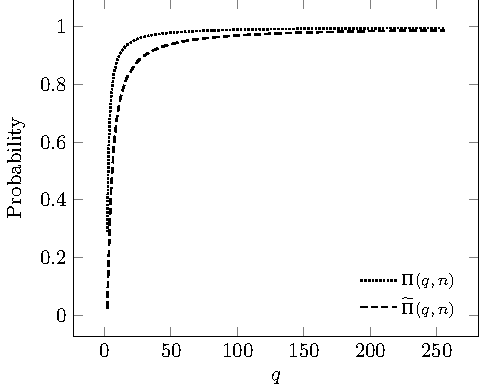
\includegraphics[width=.49\columnwidth]{charts/inv-prob/inv-prob}
  }
  \subfloat[
    Figure~\ref{fig:1a}, with $q \geq 16$.\label{fig:1b}
  ]{
    % 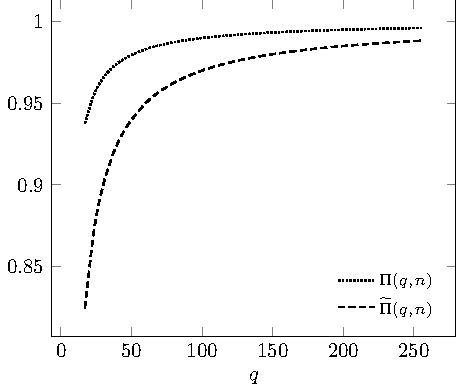
\includegraphics[width=.458\columnwidth]{charts/inv-prob/inv-prob-zoom}
  }
  \caption{Probability of obtaining an invertible matrix, populated with field
    elements where $2 \leq q \leq 256$ and $q$ is a prime power, given the
    quantity of layers of Rainbow.}\label{fig:1}
\end{figure}

It is also useful to calculate $\lim_{n \to \infty} \Pi(q, n)$ to observe
changes in the probability with the growth of the number of equations. We note that this limit is equivalent to the pentagonal number theorem due to Euler~\cite[Theorem 14.3]{Apostol:2010}. Thus, we can make use of the identity
\begin{align}
  \Pi(q) = \sum_{k = -\infty}^{\infty}
    {(-1)}^{k} q^{\frac{-3 \cdot k^{2} + k}{2}}
\end{align}
and obtain a fast approximation of the probability when $n$ tends to infinity.
We use the SageMath language, which features arbitrary precision real numbers,
to obtain these values and find out that, when $n \geq 56$,
$\Pi(q) \approx_{10^{-18}} \Pi(q, n)$ and
$\widetilde{\Pi}(q) \approx_{10^{-8}} \widetilde{\Pi}(q, n)$.
Thus, Figure~\ref{fig:1} also accurately reflects the behaviour of $\Pi(q)$,
\emph{i.e.}, current values of $n$ already reach effective upper bounds for
this probability.

If we consider that the two-dimensional coefficient matrix of $\mathcal{F}$ has
an effective size of $\frac{n^{2} + n}{2}$ due to the aforementioned monomial
ordering strategy, we note that the inversion event happens almost surely.
This evidence shows that computing a preimage in order to sign a message
happens at the first try with high probability in a wide range of Rainbow
configurations. Therefore, the cost of a central map reconfiguration, in the
case that chosen vinegar variables do not lead to an invertible central map, is
amortized by the overwhelming probability that a signature is successfully
generated.

\subsection{Similarity of multiple signatures}\label{subsec:similar}

Vinegar variables chosen to invert the central map are an integral part of the
preimage $y = \mathcal{F}^{-1}(x)$. For instance, in the case $u = 2$, these
make roughly a third of the output, considering common parameters for Rainbow.
Further, recall that there are approximately $q^v$ possibilities for $y$. Our
proposal eliminates this choice by locking vinegar variables into the private
key. Hence, it is essential to know if such variables create patterns in which
private information may leak through a multi-target attack. We use the SageMath
PRNG, which implements a front-end to the \texttt{/dev/urandom} Linux kernel
space generator.

Recall that a message digest $d$ is signed instead of the entire document.
Evidently, a secure cryptographic hash function shall produce an output that
appears to be random. The application $x = \mathcal{S}^{-1}(d)$ does not affect
this behaviour, since the map is also random. Hence, we need not simulate this
calculation in this analysis. According to Subsection~\ref{subsec:invert}, the
inversion $y = \mathcal{F}^{-1}(x)$ creates a valid preimage with overwhelming
probability, where the first $v_{1}$ elements of any $y$ are the same.

We observe the distribution of field elements in vectors after the final
function application, that is, $z = \mathcal{T}^{-1}(y)$. Let
$Z'_{t} = (z_{1}, \dots, z_{t}) \random{} \mathbb{F}_{q}^{n}, t \in \mathbb{N}$ be
a $t$-uple of ``signatures''. We build the sequence $Z_{t} = (z_{1}^{1},
z_{1}^{2}, \dots, z_{1}^{n}, z_{2}^{1}, \dots, z_{t}^{n - 1}, z_{t}^{n})$.
When part of the vector $y$ is fixed, we instead denote these by
$\widetilde{Z}'_{t}$ and $\widetilde{Z}_{t}$. Our hypothesis is that $Z_{t}$
and $\widetilde{Z}_{t}$ behave similarly to observations sampled from the
discrete uniform distribution $\mathcal{U}\{0, q - 1\}$. It is known that its
standard deviation, where $r$ values are observed in an equally likely manner,
is equal to $\sqrt{\frac{r^{2} - 1}{12}}$. We set $r = q$ in the context of $\mathbb{F}_{q}$, and thus it is expected that
\begin{align}
  \lim_{t \to \infty} \sigma(\widetilde{Z}_{t}) = \sqrt{\frac{q^{2} - 1}{12}},
\end{align}
suggesting that greater values of $n$ and $t$ approximate faster to the
theoretical standard deviation.

\begin{figure}[ht]
  \subfloat[
    $d_{\sigma}^{t}$ for $n = 42, v_{1} = 17$.\label{fig:2a}
  ]{
    % 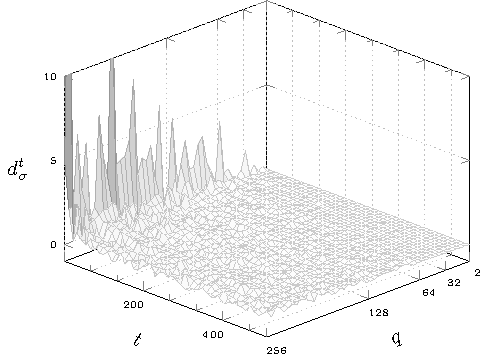
\includegraphics[width=.49\columnwidth]{charts/measure-diff/std-diff-n42}
  }
  \subfloat[
    $d_{\sigma}^{t}$ for $n = 90, v_{1} = 35$.\label{fig:2b}
  ]{
    % 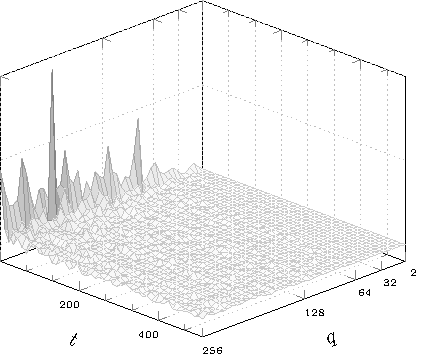
\includegraphics[width=.425\columnwidth]{charts/measure-diff/std-diff-n90}
  }
  \caption{Difference of standard deviations when $1 \leq t \leq 512$,
    and $2 \leq q \leq 256$ with $q$ as a prime power.}\label{fig:2}
\end{figure}

Let us denote the absolute difference between standard deviations for a value
$t$ as $d_{\sigma}^{t} = |\sigma(Z_{t}) - \sigma(\widetilde{Z}_{t})|$.
Figure~\ref{fig:2} shows the amplitude of such values for various values of $q$
and $t$. We note that the largest values of $d_{\sigma}^{t}$ occur for finite
fields of higher orders and lower $t$. For instance, given the vector space
$\mathbb{F}_{223}^{42}$, we have $d_{\sigma}^{1} \approx 8.25$, and for a
slightly higher $t$, we obtain a much lower value
$d_{\sigma}^{11} \approx 0.24$. This behaviour is also observed within absolute
differences of means, defined analogously as $d_{\mu}^{t}$. The vector space
$\mathbb{F}_{191}^{42}$ gives the values $d_{\mu}^{1} \approx 5.31$ and,
comparatively, $d_{\mu}^{9} \approx 1.14$.

The comparison of expected and obtained standard deviations and means in our
experiments gives positive results and confirms the law of large numbers.
Still, it is interesting to look at the diffusion of values within
$\widetilde{Z}_{t}$ and infer that it does not simply simulate the mean and
standard deviation for a known discrete uniform. We count the amount of values
for each class $0 \leq k \leq q - 1$ and refer to them by $Z_{t, k}$ and
$\widetilde{Z}_{t, k}$. By the central limit theorem, these counts should be
normally distributed.

Figure~\ref{fig:3} shows the cumulative distribution function (CDF) plot and
the Q-Q (quantile-quantile) plot for such samples. The expected CDF, as well as
examples for $Z_{t}$ and $\widetilde{Z}_{t}$, show that all values are fairly
distributed, with small variations due to the random generation of field
elements. However, we note that this is due to the low number of classes,
\emph{i.e.} the order of the finite field, and experimentally confirm that such
discrepancies are largely reduced with $q = 2^{10}$. This is further confirmed
by the Q-Q plot, which in this case is more commonly referred to as a normal probability plot. It is built by pairing the normalized counts with quantiles from the standard normal distribution. Such quantiles are called normal order statistics, or rankits~\cite{Ipsen:194405}, which are hereafter referred to as a $K$. 

Generating precise values for $K$ is non-trivial, and thus a method to yield approximate values is used. Let $r \in \mathbb{N}$ be a precision parameter. A number $rq$ of samples are taken from a standard normal distribution and organized into $q$-uples $K_{1}, \dots, K_{r}$. Then, let $\min(S, i)$ represent the $i$-th smallest value in a non-empty set $S$ with a partial order. The $q$-uple $K$ is calculated as 
\[
    K = (\mu(\{\min(K_{j}, i) : 1 \leq j \leq r\}) : 1 \leq i \leq q).
\]
We have found experimentally that the lowest precision parameter $r = 1$ is still useful to interpret the graph. The resulting plot shows that points are sufficiently close to the $y = x$ expected line.

\begin{figure}[htbp]
  \subfloat[
    CDF plot.\label{fig:3a}
  ]{
    % 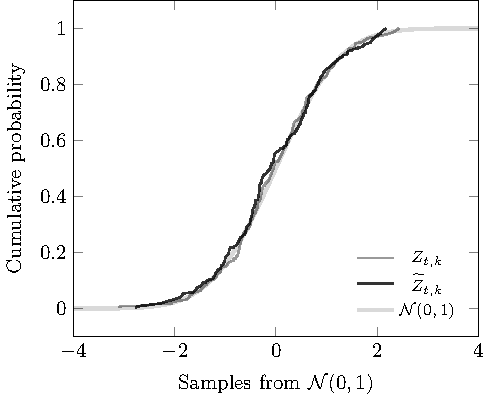
\includegraphics[width=.49\columnwidth]{charts/diffusion/cdf-plot}
  }
  \subfloat[
    Q-Q plot.\label{fig:3b}
  ]{
    % 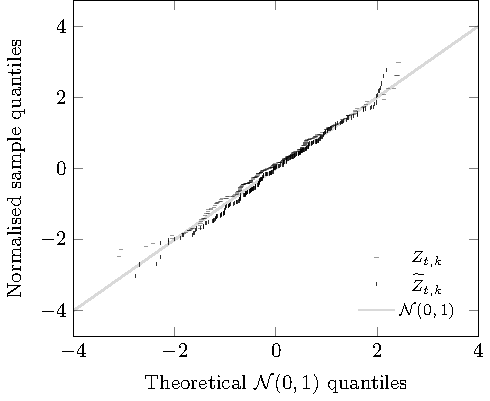
\includegraphics[width=.47\columnwidth]{charts/diffusion/qq-plot}
  }
  \caption{Distribution of counts of elements in $Z_{t}$ and
    $\widetilde{Z}_{t}$ such that $t = 2^{16}$ for
    $\mathbb{F}_{256}^{90}$.}\label{fig:3}
\end{figure}

Our argument indicates that, even if part of the preimage created by the
central map is fixed, the remaining affine map application disrupts this
pattern with high efficacy. Hence, an attacker with possession of multiple
signatures created by our method would not be more capable of forging a new
signature or deducing private information.

\subsection{Security analysis}\label{subsec:analysis}

A variety of attacks currently thwart the security of Rainbow-like signature
schemes if parameters are not chosen carefully. We briefly state each of
those, along with their estimated complexities~\cite{Petzoldt:201005},
and argue that our methods do not facilitate such attacks.

\subsubsection{Direct attack.} An attacker with possession of a digest $d$ and
the public key $\mathcal{P}$ tries to solve $\mathcal{P}(x) = d$. This is done
by fixing some of the variables and applying an algorithm built upon the theory
of Gröbner basis, such as the Hybrid approach~\cite{Bettale:201207:inproc}.
While it is hard to pinpoint the exact running time of such methods, the
authors give an estimation of its asymptotic complexity in Equation 5 of the
aforementioned work.

\subsubsection{UOV attack.} The multi-layer approach of Rainbow does not hinder
attacks that also work on the UOV signature scheme. This attack was originally
created by Kipnis and Shamir~\cite{Kipnis:199808} to break the Balanced
Oil-Vinegar scheme. The objective of this attack is to obtain an equivalent
private key by means of finding the preimage of a specific oil subspace under
the map $\mathcal{T}$. The complexity of the generalized attack for unbalanced
schemes~\cite{Kipnis:199904} is
$o_{u}^{4} \cdot q^{n - 1 - 2 \cdot o_{u}}$ field multiplications.

\subsubsection{MinRank attack.} All systems of polynomials in the public key
$\mathcal{P}$ may be individually represented as matrices. This attack
consists in finding linear combinations of these, such that they have a lesser
rank than $v_{2}$, in the case of Rainbow. This allows an attacker to isolate
the central map polynomials from the first layer of Rainbow, and analogously
recover the remaining layers with a much lower effort. In the context of
Rainbow~\cite{Billet:200609}, its complexity is
$q^{v_{1} + 1} \cdot m \cdot (\frac{n^{2}}{2} - \frac{m^{2}}{6})$ field
multiplications.

\subsubsection{HighRank attack.} In a similar way to MinRank, linear
combinations of public key matrices are used to find the variables which
appear the lowest number of times in the central map. This is used to identify
the last Rainbow layer, and obtain the previous layers similarly. The
complexity of the improved attack~\cite{Ding:200806} is
$q^{o_{u}} \cdot \frac{n^{3}}{6}$ field multiplications.

\subsubsection{Rainbow-Band-Separation attack.} An extension of the
UOV-Reconciliation attack by the same authors~\cite{Ding:200806} that
targets Rainbow, with the intent of producing an equivalent private key. It
explores the fact that the central map matrix representation is composed of
zeroes on its lower right corner. These yield quadratic equations which, if
solved, lead to an alternative private key. The complexity of this attack is
given by the hardness of solving a large system of equations, as seen
above, is hard to estimate.

\subsubsection{Side-channel attacks.} It may be observed that none of the
proposed Rainbow variants, as well as the original scheme, present constant
time signature generation algorithms. Particularly, in Rainbow-$\eta_2$, a
considerable amount of computation is added to the signature algorithm when one
of the systems is not solvable. In a chosen message attack, one may observe the
time spent on multiple signature generation steps and easily check if the
linear systems are solvable, thus obtaining information about the central map.
Although there are no known attacks that make use of this technique, it is
possible that there may exist information leaks when applying our methods to
Rainbow-like schemes.

\paragraph{} We do not discard the possibility that specialized attacks exist,
particularly ones that take in account multiple signatures, due to our fixing
of vinegar variables. However, we have seen in Subsection~\ref{subsec:similar}
that signatures generated by our method are comparably random with respect to
conventional Rainbow signatures. Furthermore, we note that most attacks look
for special structures within the private key. While our methods indeed modify
the private key representation, it is still present in its entirety on the
public key composition, which is the only information available to malicious
entities that can be possibly used to forge signatures. We thus suggest that
the right choice of parameters is made whenever our methods are applied,
\emph{e.g.} according to~\cite{Petzoldt:201005}, to protect the scheme
instance against these attacks.

\section{Enhancement of existing schemes}\label{sec:experiments}

Our method does not depend on special structures inserted on the private key.
Consequently, it can be applied to all known Rainbow-like schemes. We
experiment with several sets of parameters and observe the reduction of private
keys. It is known that there are various limitations for the choice of
parameters that lead to secure instances of
Rainbow~\cite{Petzoldt:201005}. We implement several known guidelines
and confirm that our proposal does indeed work for a large range of parameters.
However, we only show results for known secure parameter sets to prevent
accidental endorsement of untested, and possibly insecure, instances.

\begin{table}[htbp]
  \renewcommand{\arraystretch}{1.2}
  \setlength{\tabcolsep}{6.5pt}
  \centering
  \caption{Reduction of Rainbow key sizes, in bytes, for various instances of the scheme.}\label{tab:1}
  \begin{tabular}{*{2}{l}*{5}{r}}
    \toprule
    Instance & Parameters & $n$ & $m$ & $|\mathcal{K}_{Pr}|$ & $|\mathcal{K}_{Pr} ^{\eta}|$ & Difference \\ \midrule
    I-a    & $(\mathbb{F}_{ 16}, 32, 32, 32)$  &   96 &   64 &   100208 &   33152 & $-66.92\%$ \\
    I-b    & $(\mathbb{F}_{ 31}, 36, 28, 28)$  &   92 &   56 &   114308 &   31676 & $-72.29\%$ \\
    I-c    & $(\mathbb{F}_{256}, 40, 24, 24)$  &   88 &   48 &   143384 &   33024 & $-76.97\%$ \\
    III-b  & $(\mathbb{F}_{ 31}, 64, 32, 48)$  &  144 &   80 &   409463 &   87628 & $-78.60\%$ \\
    III-c  & $(\mathbb{F}_{256}, 68, 36, 36)$  &  140 &   72 &   537780 &   99656 & $-81.47\%$ \\
    IV-a   & $(\mathbb{F}_{ 16}, 56, 48, 48)$  &  152 &   96 &   376140 &  103336 & $-72.53\%$ \\
    V-c    & $(\mathbb{F}_{256}, 92, 48, 48)$  &  188 &   96 &  1274316 &  218984 & $-82.82\%$ \\
    VI-a   & $(\mathbb{F}_{ 16}, 76, 64, 64)$  &  204 &  128 &   892078 &  233044 & $-73.88\%$ \\
    VI-b   & $(\mathbb{F}_{ 31}, 84, 56, 56)$  &  196 &  112 &  1016868 &  217244 & $-78.64\%$ \\
    P-080  & $(\mathbb{F}_{256}, 17, 17,  9)$  &   43 &   26 &    19208 &    5914 & $-69.21\%$ \\
    P-100  & $(\mathbb{F}_{256}, 26, 22, 21)$  &   69 &   43 &    75440 &   23193 & $-69.26\%$ \\
    P-128  & $(\mathbb{F}_{256}, 36, 28, 15)$  &   79 &   43 &   103704 &   22110 & $-78.68\%$ \\
    P-192  & $(\mathbb{F}_{256}, 63, 46, 22)$  &  131 &   68 &   440638 &   71773 & $-83.71\%$ \\
    P-256  & $(\mathbb{F}_{256}, 85, 63, 30)$  &  178 &   93 &  1086971 &  164721 & $-84.85\%$ \\
    \bottomrule
  \end{tabular}
\end{table}

We show results for the application of our method in Table~\ref{tab:1},
considering the following Rainbow instances. Conservative choices were made by
the Rainbow submission authors~\cite{Ding:201712} to fit security
categories as requested by NIST\@. We apply our method to these recent
proposals, and additionally
choose parameters from Petzoldt~\cite[Table 6.12]{Petzoldt:201307} for
further comparison. The latter are named P-$\ell$, where $\ell$ is the security
level in bits. Indeed, the choice of $v_{1}$ remarkably affects the results.
Moreover, a minimal value of $o_{u}$ is also known to further reduce the
private key size. Indeed, we suggest that $v_{1} \geq o_{u}$ as much as
possible to maximize the results of our method. However, we remark that one
must set sufficient parameters for $o_{i}$ such that the scheme still resists
direct and UOV attacks.

The case of Rainbow variants is slightly more convoluted. Schemes claim
optimizations of the private key often through the inclusion of inner
structuring. To measure the impact of our method within the context of these
schemes, it is imperative to understand such structures. For instance, it may
be the case that a method introduces sparseness related to specific vinegar
variables. Thus, the reduction would not be equally distributed over the
private key elements and, as such, our method would have its efficiency
reduced.

To the best of our knowledge, it is not trivial to combine our strategy with the schemes presented in Subsection~\ref{subsec:priv}, and resulting gains would be evidently reduced. Furthermore, several of those schemes were subsequently broken or new parameters were proposed, suggesting that such a combination would not be productive. We
thus consider only schemes that reduce the public key size, \emph{i.e.}
CyclicRainbow~\cite{Petzoldt:201012} and
RainbowLRS2~\cite[Section 9.2]{Petzoldt:201307}.

\begin{table}[htbp]
  \renewcommand{\arraystretch}{1.2}
  \centering
  \caption{Total reduction of Rainbow key pairs, in bytes, for variants of the scheme.}\label{tab:2}
  \begin{tabular}{*{2}{l}*{5}{r}}
    \toprule
    Instance & Parameters & Variant & $|\mathcal{K}_{Pr}|$ & $|\mathcal{K}_{Pr} ^{\eta}|$ & $|\mathcal{K}_{Pu}|$ & Difference \\ \midrule
    \multirow{3}{*}{P-080}  & \multirow{3}{*}{$(\mathbb{F}_{256}, 17, 13, 13)$}  &  Classic &  \multirow{3}{*}{ 19546} &  \multirow{3}{*}{ 6524} &   25740 & $-28.76\%$ \\
                            &                                                    &   Cyclic &                          &                         &   10618 & $-62.15\%$ \\
                            &                                                    &     LRS2 &                          &                         &    9789 & $-63.98\%$ \\
    \multirow{3}{*}{P-100}  & \multirow{3}{*}{$(\mathbb{F}_{256}, 26, 16, 17)$}  &  Classic &  \multirow{3}{*}{ 46131} &  \multirow{3}{*}{12474} &   60390 & $-31.60\%$ \\
                            &                                                    &   Cyclic &                          &                         &   22246 & $-67.41\%$ \\
                            &                                                    &     LRS2 &                          &                         &   20662 & $-68.89\%$ \\
    \multirow{3}{*}{P-128}  & \multirow{3}{*}{$(\mathbb{F}_{256}, 36, 21, 22)$}  &  Classic &  \multirow{3}{*}{105006} &  \multirow{3}{*}{24924} &  139320 & $-32.78\%$ \\
                            &                                                    &   Cyclic &                          &                         &   48411 & $-69.98\%$ \\
                            &                                                    &     LRS2 &                          &                         &   45547 & $-71.16\%$ \\
    \bottomrule
  \end{tabular}
\end{table}

We compare the total key pair sizes $|\mathcal{K}_{Pr}| + |\mathcal{K}_{Pu}|$
when our method is used alongside Rainbow variants that reduce the public key
size. Table~\ref{tab:2} shows the quantity of field elements for sets of
parameters from Petzoldt~\cite[Table 9.8]{Petzoldt:201307}. We calculate
$|\mathcal{K}_{Pu}|$ for the variants according to Equations 9.2 and 9.4 of the
same work, and as per its Remark 9.1, we note that $q = 16$ and $q = 31$ are not
considered due to a security restriction of RainbowLRS2. We obtain positive
results, with key pair size reductions of up to factors of 3 and no security
harm to the resulting scheme.

The use of CyclicRainbow or RainbowLRS2 with the Rainbow-$\eta_{2}$ method is
recommended. These variants are based on the linear relations described in
Subsection~\ref{subsec:scheme}, and resulting implementations may be
effortlessly modified to use our proposal. Moreover, in the case that higher
parameters are needed, \emph{e.g.} a security level of $256$ bits, we note that
the key pair is reduced more aggressively. Thus, our results reflect
changes over a wide variety of platforms and possible Rainbow deployments that
benefit from lower storage requirements.

We also briefly discuss the effect of these changes on the signature generation
step overall performance. In the case of Rainbow-$\eta_{1}$, it does not vary
greatly due to the fast regeneration of the central map elements from a given
PRNG and $\mathbf{S}$. On the other hand, Rainbow-$\eta_{2}$ uses elaborate
techniques to reconstruct the central map if vinegar variables are not
suitable.  This process is not without cost, and it may negatively affect the
average signature generation time. Still, by making use of Rainbow-$\eta_{3}$,
these computations are entirely avoided by choosing a new salt instead of new
vinegar variables, reducing the inherent overhead.

\bibliographystyle{alpha}
\bibliography{ref}

\end{document}
